
\subsection*{\textbf{Question 1.b)}}
\begin{quote}

\textbf{Problem}
\begin{quote}Now use the Box-Muller method to generate 1000 normally-distributed random numbers. To check if they are following the expected Gaussian distribution, make a histogram (scaled appropriate) with the corresponding true probability distribution (normalized to integrate to 1) as line. This plot should contain the interval of -5$\sigma$ until $5\sigma$ from the theoretical probability distribution. Indicate the theoretical $1\sigma$, $2\sigma$, $3\sigma$ and $4\sigma$ interval with a line. For this plot, use $\mu =3$ and $\sigma = 2.4$ and choose bins that are appropriate.
\end{quote}

\textbf{Solution} 



\begin{quote}
The solution consists of deriving the  transformation of two i.i.d uniform variables to two i.i.d normal distributed variables with the Box-Muller method. A brief version of the derivation can be found below. The final transformation, equation \ref{EQ:boxmuller}, is  implemented in the random number generator and used to generate the plot. The final histogram is created with 20 bins and can be found on page \pageref{fig:normal}.
\\


Let $X, Y \sim G(\mu, \sigma ^2)$ be two i.i.d Gaussian distributed random variables. Their joined CDF is then given by, 
\begin{equation}
P(X \leq x_1, Y \leq y_1) =  \int_{-\infty}^{x_1} \int_{-\infty}^{y_1} G(x| \mu, \sigma^2) G(y| \mu, \sigma^2) dx dy
\end{equation}

Transforming to polar coordinates by substituting $ (x-\mu) = r \cos(\theta)$ and $ (y-\mu) = r\sin(\theta)$ yields,

\begin{align*}
P(R \leq r_1, \Theta \leq \theta_1) &= \int_0^{r_1} \int_{0}^{\theta_1} G(r\cos(\theta) \sigma + \mu| \mu, \sigma^2) G(r\sin(\theta) \sigma + \mu| \mu, \sigma^2) r dr d\theta \\
&= \frac{1}{2 \pi \sigma^2} \int_0^{r_1} \int_{0}^{\theta_1} re^{ -\frac{1}{2} \left[ \left( \frac{r\cos(\theta)}{\sigma} \right)^2  + \left( \frac{r\sin(\theta)}{\sigma} \right)^2 \right]}  dr d\theta \\
&=  \frac{1}{2 \pi \sigma^2} \int_0^{r_1} \int_{0}^{\theta_1} re^{ -\frac{r^2}{2 \sigma ^2} } dr d\theta
\end{align*}

The CDF's  for the polar coordinates are now given by, % $R$ and $\theta$ are now given by, 

\begin{align}
P(R \leq r_1) &= \frac{1}{\sigma^2} \int_{0}^{r_1}  re^{ -\frac{r^2}{2 \sigma ^2} } dr =  \int_{0}^{r_1} \frac{d}{dr} \left( -e^{ -\frac{r^2}{2 \sigma ^2}}  \right) dr = 1 - e^{- \frac{r_1^2}{2 \sigma^2}} \\
P(\Theta \leq \theta_1) &= \frac{1}{2 \pi }  \left[ -e^{-\frac{r^2}{2 \sigma^2}} \right]^{\infty}_{0} \int_{0}^{\theta_1} d\theta = \frac{\theta_1}{2\pi}
\end{align}

The CDFs can be used to convert  two uniform distributed variables to the polar coordinates of the Gaussian distributed variables. Let $U_1, U_2 \sim U(0,1)$ be two i.i.d uniform variables. From the transformation law of probability we then must have that, %The transformation law of probability then states that,

\begin{align}
P(R \leq r_1) &= P(U_1 \leq u_1) \rightarrow  1 - e^{- \frac{r_1^2}{2\sigma^2}}  = \int_{0}^{u1} du_1 = u_1 \\
P(\Theta \leq \theta) &= P(U_2 \leq u_2) \rightarrow   \frac{\theta_1}{2\pi} = \int_{0}^{u2} du_2 = u_2 
\end{align}

The transformation from the two uniform distributed variables to the polar coordinates of the Gaussian distributed variables then becomes,

\begin{align}
r_1 &=  \sqrt{-2\sigma^2 \ln(1 - u_1)} \\
\theta_1 &= 2 \pi u_2
\end{align}

Converting back to Cartesian coordinates  yields the transformation from two i.i.d uniform distributed variables to two i.i.d Gaussian distributed variables;
\begin{align}
x_1 &= r\cos(\theta) + \mu = \sqrt{-2\sigma^2 \ln(1 - u_1)} \cos( 2 \pi u_2 ) + \mu \\
y_1 &= r\sin(\theta) + \mu = \sqrt{-2\sigma^2 \ln(1 - u_1)} \sin( 2 \pi u_2 ) + \mu
\label{EQ:boxmuller}
\end{align}
\\
\\
These above transformation are implemented in  the random number generator (see page \pageref{CODE:RNG}).  The code for the generation of the plot and the created plot can be found below. The code that generates the plot makes besides the RNG use of a function for the normal distribution in the file \texttt{./Code/mathlib/statistics.py}. This file is treated as a shared module and can be found on page 22. The called function, \texttt{normal}, can be found on line 227 in this file.


\end{quote}

\textbf{Code - Plots}

\begin{quote}
The code for generating the plots. The imports are again not explicit shown, but can be found on page 19. The shared modules can be found on pages 19 and 22. 


\lstinputlisting[firstline=68,lastline=122]{./Code/assigment_1.py}
\end{quote}


\textbf{Code - Output plot(s)}
\vspace*{-0.5cm}
\begin{quote}
\begin{figure}[!hb]
\centering
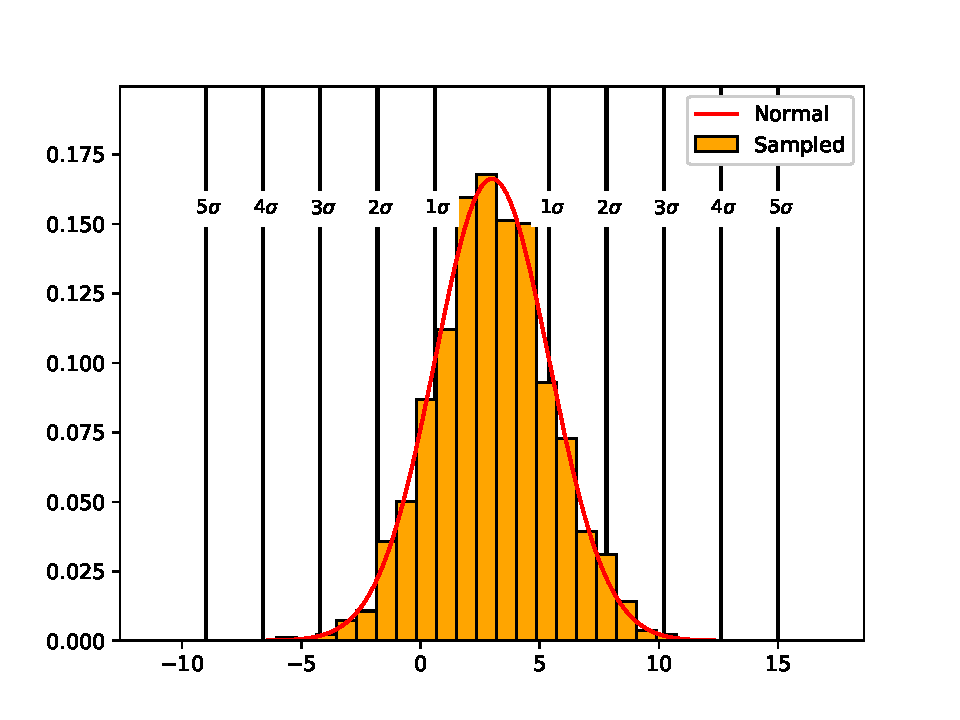
\includegraphics[width=13cm, height=7.0cm]{./Plots/1_hist_gaussian.pdf}
\caption{A histogram of the 1000 random normal distributed variables generated with the box muller method for $\mu = 3$ and $\sigma = 2.4$  (orange). The red line is the true normal distribution.  The histogram appears to approximate the distribution quite well, but displays small deviations. The bin left of the peak (the highest bin) is larger than it should be. The first bins right of the peak is smaller than it should be and the second bin right of the peak is to high.  The histogram does however still appear to be acceptable by eye. A statistical test is of course better to determine whether the histogram would truly be acceptable or not.}
\label{fig:normal}
\end{figure}
\end{quote}
\end{quote}

%\textbf{Code - output } 
%\begin{quote}
% The code that produces the output.
%\lstinputlisting{./code/assigment1_a.py}
%\end{quote}

%\textbf{Code - helper } 
%\begin{quote}
%The code for the Poisson distribution and the factorial function.  
%\lstinputlisting[firstline=2,lastline=46]{./code/mathlib/utils.py}
%\end{quote}


%\textbf{Output}
%\begin{quote}
%The output produced by \textsf{/code/assigment1\_ a.py} 
%\lstinputlisting{./output/assigment1_a_out.txt}
%\end{quote}











